\documentclass[12pt]{article}
\usepackage{graphicx}
\usepackage{geometry}
\geometry{margin=1in}
\usepackage{caption}

\title{\textbf{Smart Thermostat Project Submission}}
\author{Scott Nguyen}
\date{\today}

\begin{document}
	\maketitle
	
	\section{How to Run the Project}
	\begin{enumerate}
		\item Extract the provided \texttt{project.tgz} archive:
		\begin{verbatim}
			tar -xzvf project.tgz
			cd thermostat_project_folder
		\end{verbatim}
		\item Make sure \texttt{project.sh} is executable:
		\begin{verbatim}
			chmod +x project.sh
		\end{verbatim}
		\item Launch the host server and QEMU virtual machine:
		\begin{verbatim}
			./project.sh
		\end{verbatim}
		This script:
		\begin{itemize}
			\item Starts \texttt{server.py} on the host (port 8000).
			\item Boots the QEMU ARM VM with the thermostat client running automatically.
		\end{itemize}
	\end{enumerate}
	
	\section{Verification Steps}
	\subsection{1. Server Receives Status Updates}
	The host \texttt{server.log} shows regular POST requests from the VM client to the \texttt{/status} endpoint every 5 seconds.
	\begin{figure}[h!]
		\centering
		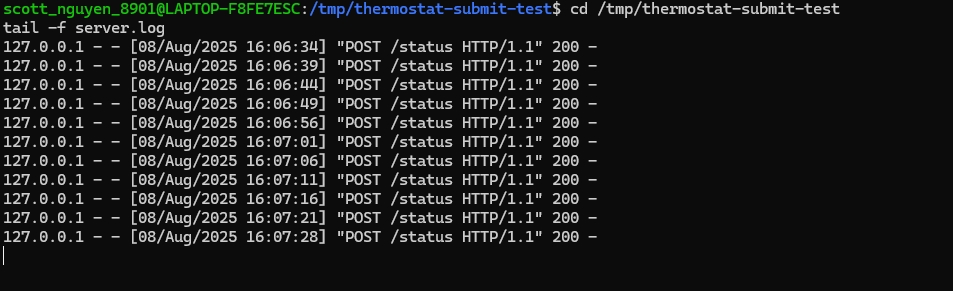
\includegraphics[width=0.85\linewidth]{server-log.png}
		\caption{Regular status updates sent from VM client to server.}
	\end{figure}
	
	\subsection{2. Remote Schedule Update via HTTP POST}
	A new temperature program is sent from the host to the VM using:
	\begin{verbatim}
		curl -X POST http://127.0.0.1:8000/program \
		-H "Content-Type: application/json" \
		-d '[{"time":"00:00","temp":72},
		{"time":"08:00","temp":68},
		{"time":"22:00","temp":65}]'
	\end{verbatim}
	\begin{figure}[h!]
		\centering
		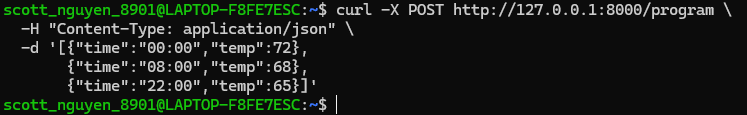
\includegraphics[width=0.85\linewidth]{curl-post.png}
		\caption{Host sends updated program to the thermostat client.}
	\end{figure}
	
	\subsection{3. Heater Control Log in VM}
	Inside the VM:
	\begin{verbatim}
		tail -f /var/log/heater
	\end{verbatim}
	The log shows the heater turning \texttt{on} and \texttt{off} based on temperature readings.
	\begin{figure}[h!]
		\centering
		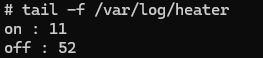
\includegraphics[width=0.5\linewidth]{heater.png}
		\caption{Heater on/off events with timestamps.}
	\end{figure}
	
	\subsection{4. Simulated Temperature Readings in VM}
	The thermostat reads from \texttt{/tmp/temp} (simulated thermocouple). This can be observed with:
	\begin{verbatim}
		watch -n 1 cat /tmp/temp
	\end{verbatim}
	\begin{figure}[h!]
		\centering
		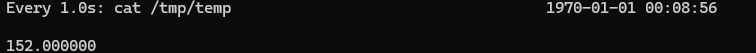
\includegraphics[width=0.65\linewidth]{watch-cat-temp.png}
		\caption{Simulated temperature readings inside VM.}
	\end{figure}
	
	\subsection{5. Post-Update Confirmation in Server Log}
	After sending a new program, the server log confirms receipt with a \texttt{POST /program} entry.
	\begin{figure}[h!]
		\centering
		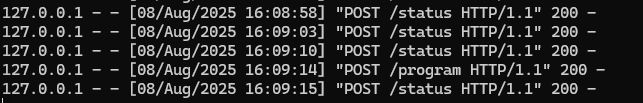
\includegraphics[width=0.85\linewidth]{post-update.png}
		\caption{Server confirms program update from host.}
	\end{figure}
	
	\section{Conclusion}
	The tests confirm that:
	\begin{itemize}
		\item The thermostat client starts automatically in the VM.
		\item The client reads simulated temperature data.
		\item Heater control logic works and logs actions.
		\item Status is reported to the host server.
		\item Remote schedule updates are accepted and applied.
	\end{itemize}
	This satisfies the core requirements for the Smart Thermostat IoT project.
\end{document}
